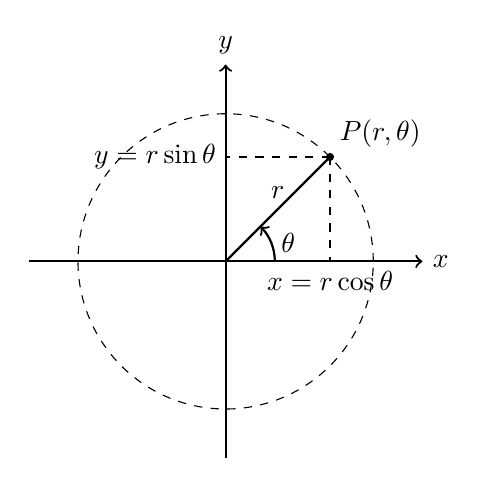
\begin{tikzpicture}[scale=1.25]

    % Draw Cartesian axes
    \draw[->, thick] (-2, 0) -- (2, 0) node[right]{$x$};
    \draw[->, thick] (0, -2) -- (0, 2) node[above]{$y$};

    % Draw a circle to represent the radial distance
    \draw[dashed] (0, 0) circle (1.5);

    % Draw the angle θ
    \draw[->, thick] (0.5, 0) arc (0:45:0.5) node[midway, right]{$\theta$};

    % Draw the radial line
    \draw[thick] (0, 0) -- (45:1.5) node[midway, above]{$r$};

    % Mark the point P(r, θ)
    \filldraw (45:1.5) circle (1pt) node[above right]{$P(r, \theta)$};

    % Draw dashed lines to show projections onto Cartesian axes
    \draw[dashed] (45:1.5) -- ({1.5*cos(45)}, 0) node[below]{$x = r \cos \theta$};
    \draw[dashed] (45:1.5) -- (0, {1.5*sin(45)}) node[left]{$y = r \sin \theta$};

\end{tikzpicture}